\chapter{Modelling of Wind Turbine Generators}
\label{ch: Models}

Due to huge variety of wind turbine generators and their different characteristics, modelling each machine of a wind power plant separately would be a long and exhaustive work. To address this problem, studies such as \cite{Muljadi2008}, \cite{Ellis2011}, \cite{council2008wecc} and \cite{Asmine2011}, conducted specially by the Institute of Electrical and Electronics Engineers (IEEE) and the Western Electricity Coordinating Council (WECC), developed generic models able to predict the behaviour of entire wind power plants. Such models reduced the problem complexity, since they were composed of a single equivalent generator. A two-machine model is needed only in rare cases, such as when the wind power plant is composed of two or more types of wind turbines \cite{Ellis2011}.

\section{Generic Models of Wind Turbine Generators}

The studies mentioned above have concluded that commercial wind turbine generators could be sorted into four basic types, according to their characteristics and technologies \cite{Ellis2011}. These types are described in the following subsections.

\subsection{Type-1: Squirrel Cage Induction Generator (SCIG)}

The first type of wind turbine generator is composed of a Squirrel Cage Induction Generator (SCIG) connected to a wind turbine through a controlled gearbox, as displayed in Figure \ref{fig: WTG1}.

\begin{figure}[h]
	\caption{Representation of Type-1 Wind Turbine Generator}
	\begin{center}
		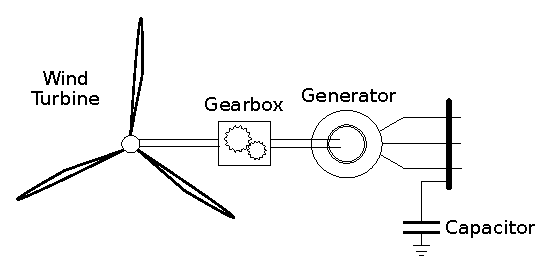
\includegraphics[scale=.8]{Images/Type1WTG.eps}
	\end{center}
	\label{fig: WTG1}
\end{figure}

Due to its torque-speed characteristics, generators of this type operate at constant rotor speed, requiring robust controllers on gearbox and blade. Besides, as usual to any induction generator, the SCIG absorbs reactive power during operation. Thus, capacitors are often employed for power factor correction purposes. Moreover, type-1 generators limit aerodynamic power by varying the pitch angle of their blades, imposing great mechanical stress on blades, shafts and gears, demanding a robust mechanical design and preventing these generators to operate above certain wind speed \cite{Ellis2011}. 

\subsection{Type-2: Wound Rotor Induction Generator (WRIG)}

Similarly to Type-1 WTG, Type-2 Wind Turbine Generators are composed of an asynchronous machine connected to a wind turbine via gearbox. However, instead of SCIG, Wound Rotor Induction Generator (WRIG) are used to convert kinetic energy into electricity. Generators of this type grant access to the rotor windings, allowing variances on the rotor resistance. As a direct consequence, this machine can operate in different wind speeds by adjusting its torque-speed curve as needed \cite{Ellis2011}. Therefore, Type-2 WTG have a WRIG with a variable resistance connected to its rotor terminals, as shown in Figure \ref{fig: WTG2}.

\begin{figure}[h]
	\caption{Representation of Type-2 Wind Turbine Generator}
	\begin{center}
		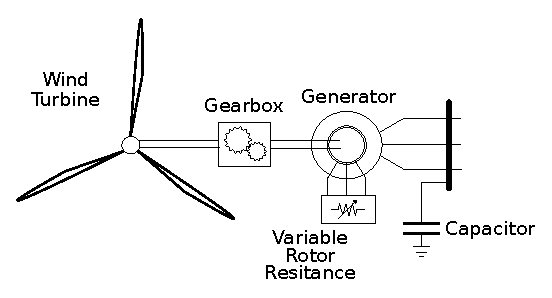
\includegraphics[scale=.8]{Images/Type2WTG.eps}
	\end{center}
	\label{fig: WTG2}
\end{figure}

Thus, this type of generator has three speed control systems, with rotor resistance control responding to rapid changes in speed, gearbox control for medium variations and pitch control for slow changes. These control systems work together to maintain power output at the desired level and reduce mechanical stress on components. The effects on the torque-speed curve caused by different rotor resistances are shown in Figure \ref{fig: Tw}.

\begin{figure}[h]
	\caption{Torque-speed curve}
	\begin{center}
		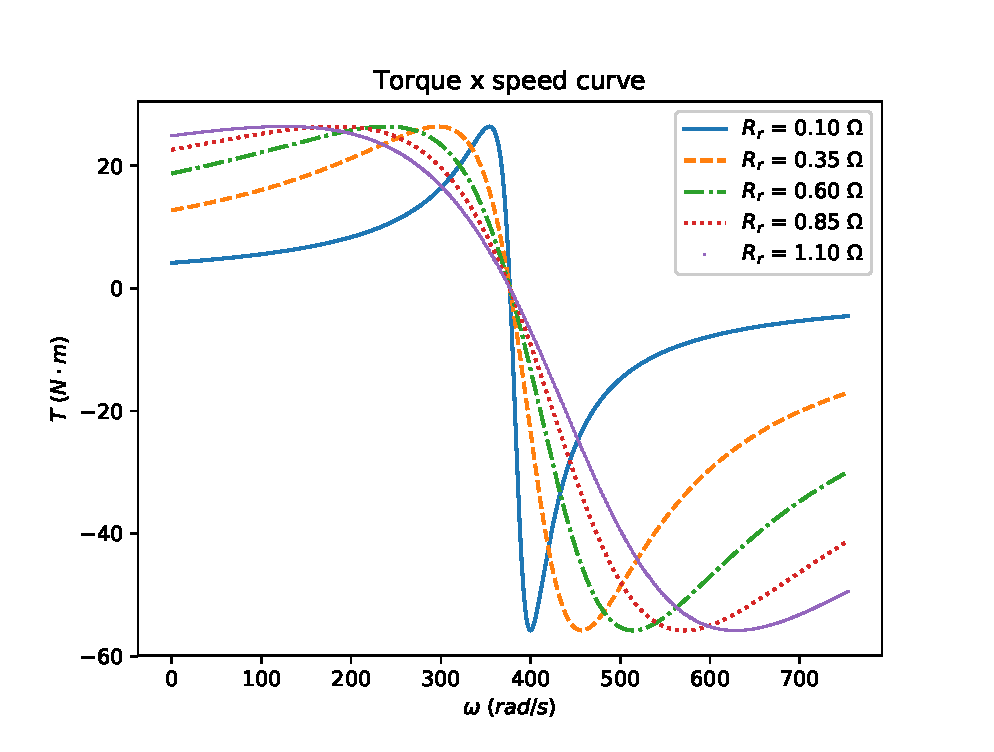
\includegraphics[scale=.6]{Images/Tw_curve.eps}
	\end{center}
	\label{fig: Tw}
\end{figure}

For a fixed power, increasing rotor resistance increases the speed needed on the shaft, allowing the wind turbine to operate above rated wind speed. However, the speed range is only $\pm 10\%$ of rated slip. Also, this machine still needs a reactive compensation circuit on its terminals, since it naturally drains reactive power from the grid \cite{Muljadi2010}.

\subsection{Type-3: Doubly Fed Induction Generator (DFIG)}

A Type-3 Wind Turbine Generator, often called Doubly Fed Induction Generator (DFIG), is also composed of a wound rotor machine connected to a wind turbine. But, instead of having a variable resistance connected to its rotor terminals, as the previous WTG type, DFIGs have their rotor windings supplied with AC voltage by a back-to-back frequency converter, as displayed in Figure \ref{fig: WTG3}. 

\begin{figure}[h]
	\caption{Representation of Type-3 Wind Turbine Generator}
	\begin{center}
		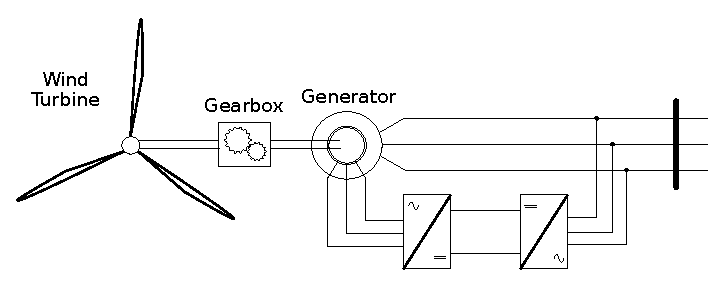
\includegraphics[scale=.8]{Images/Type3WTG.eps}
	\end{center}
	\label{fig: WTG3}
\end{figure}

The line-side converter (LSC) main purpose is to maintain voltage level on the DC link and provide reactive current during fault, while the rotor-side converter (RSC) controls active and reactive power generated by the machine by emulating different voltage frequencies on the rotor windings. By varying voltage frequency on the rotor circuit, this type of generator is able to supply power to the grid in a wider range of wind speed, reaching $\pm 30\%$ of rated slip. In addition, as result of the independent control of active and reactive power, reactive compensator circuits are no longer needed\cite{Muljadi2010}.

Since approximately $30\%$ of rated power flows through the rotor windings, power electronics components have lower specifications and do not have great impact on overall costs. On the other hand, these generators need regular maintenance due to slip rings, brushes and gearbox, preventing its broad use in offshore applications \cite{Yaramasu2015}.

\subsection{Type-4: Full-Converter Generator}

The last type of wind turbine generator, also called Full-Converter Generator, is composed of an electrical machine connected to the grid through a back-to-back frequency converter. The converters operate by controlling the frequency of the generated voltage so it matches the grid standard frequency. In this configuration, WTGs are able to produce energy in a large range of wind speed (up to almost 100\% of rated slip). Also, the connection between rotor and wind turbine shaft can be made directly or via gearbox. Likewise, it allows the use of both synchronous and asynchronous electrical machines as generator, with Permanent Magnet Synchronous Generator (PMSG), Electrical Excited Synchronous Generator (EESG) and SCIG being the most common, due to cost and maintenance purposes. Similar to DFIG, full-converter generators are able to independently control real and reactive power injected into or drained from the grid. However, since the entire generated power must flow through the power electronic devices, the overall cost of these generators is usually higher than other WTG types \cite{Yaramasu2015}. Figure \ref{fig: WTG4} depicts a typical Type-4 Wind Turbine Generator.

\begin{figure}[h]
	\caption{Representation of Type-4 Wind Turbine Generator}
	\begin{center}
		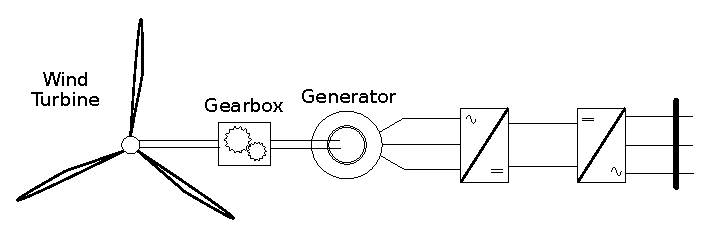
\includegraphics[scale=.8]{Images/Type4WTG.eps}
	\end{center}
	\label{fig: WTG4}
\end{figure}

Figure \ref{fig: WindShare} shows the evolution of share in installed capacity onshore for each generator type. The data shows how SCIG and WRIG lost space in the segment and how participation of DFIG and Full-Converter Generators rose, dominating the global market \cite{Magagna2017}.

\begin{figure}[h]
	\caption{Share of installed capacity for each wind turbine generator type}
	\begin{center}
		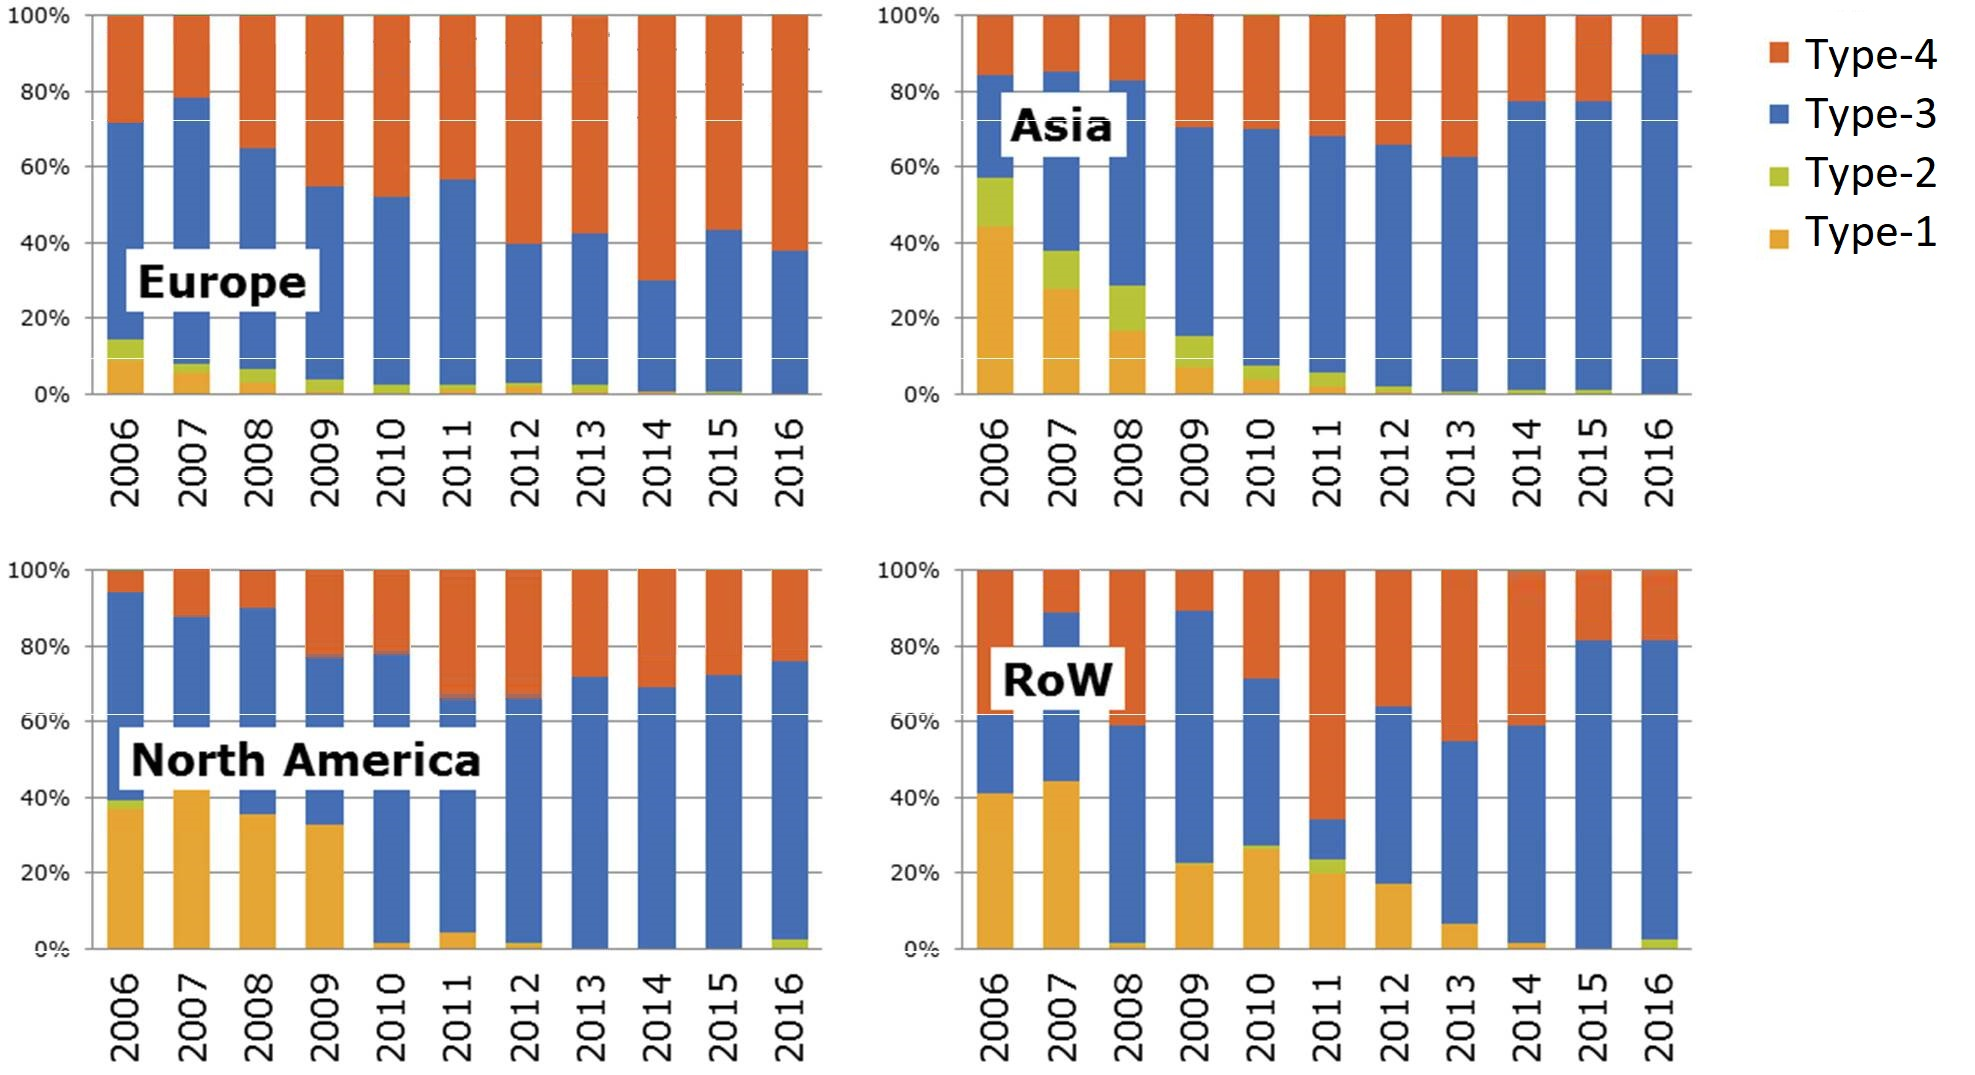
\includegraphics[scale=.2]{Images/WTGTypes.jpg}
	\end{center}
	\legend{Source: Adapted from \cite{Magagna2017}}
	\label{fig: WindShare}
\end{figure}

\section{Wind Power Plant Model Selected for Parameter Estimation}
\label{sec: WPP_model}

Many mathematical models were developed during the last years that are able to represent wind turbine generators of all types. All those models have in common the fact that they are based on the generic models proposed by the studies made by WECC and IEEE and presented in the last section. The mathematical model selected for this work is presented in this section.

Initially proposed by \cite{Erlich2012}, this mathematical model is able to represent the dynamic behaviour of both Type-3 and -4 WTGs and can be applied on simulation of entire wind power plants. Since this model is used for transient stability studies, it is assumed that wind speed and, consequently, mechanical power are constant during that interval.

In this model, WPPs are represented by their Thevenin equivalent, composed of a voltage source connected to the grid by an impedance. The direct and quadrature components of the equivalent voltage source are controlled by a series of blocks that simulate the controllers of WTGs. The block diagram of this model is shown in Figure \ref{fig: ErlMod},

\begin{figure}[h]
	\caption{WPP model proposed by Erlich}
	\begin{center}
		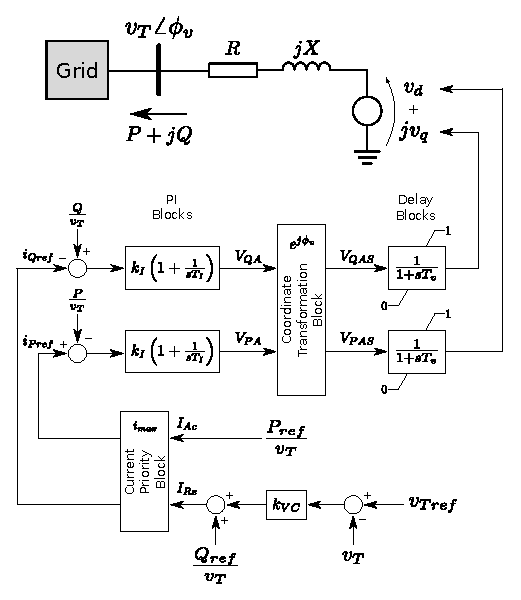
\includegraphics[scale=1]{Images/ErlichModel.eps}
	\end{center}
	\label{fig: ErlMod}
	\legend{Source: Adapted from \cite{Erlich2012}}
\end{figure}

\noindent where $v_{T}$ and $\phi_{v}$ correspond to the voltage magnitude and angle at substation bus, $P$ and $Q$ are the active and reactive power generated by the WPP, $v_{d}$ and $v_{q}$ stand for the direct and quadrature components of the generated voltage, $R$ and $X$ correspond to the Thevenin equivalent resistance and reactance, $k_{I}$ and $T_{I}$ are the PI block gain and time constant, $T_{V}$ is the delay block time constant and $k_{VC}$ is the voltage block gain.

The reference values of bus voltage ($v_{Tref}$), active ($P_{ref}$) and reactive power ($Q_{ref}$) are obtained during regime and vary according to wind speed. The real and imaginary current components that WPP must provide in order to maintain voltage and power at the reference level can be easily obtained by the equations below.

\begin{equation}
	\begin{cases}
		I_{Ac} = \frac{P_{ref}}{v_{T}} \\
		I_{Re} = k_{VC}(v_{Tref} - v_{T}) + \frac{Q_{ref}}{v_{T}}
	\end{cases}
	\label{eq: Currents}
\end{equation}

However, under certain conditions, those current components must be prioritized. System conditions are analysed by a current priority block, which limits the current previously calculated by checking if it surpasses the limits allowed and if terminal voltage is below a threshold value $v^{*}$, characterizing voltage sag. Figure \ref{fig: CurrentPriority} exemplifies the block operation.

\begin{figure}[b]
	\caption{Current priority operation}
	\centering
	\begin{subfigure}[b]{0.4\textwidth}
		\centering
        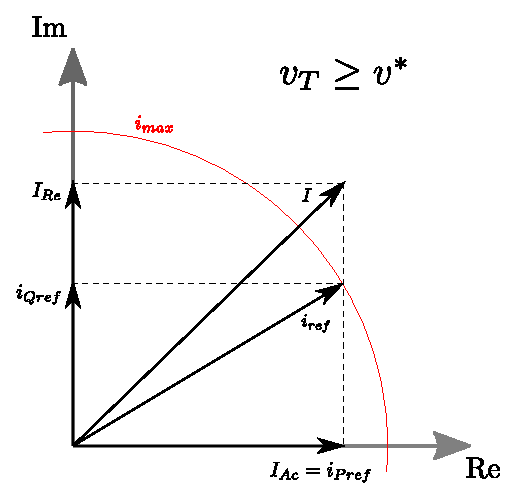
\includegraphics[width=\textwidth]{Images/priority_block1.eps}
        \caption{during normal conditions}
        \label{fig: priority_normal}
	\end{subfigure}
    \begin{subfigure}[b]{0.45\textwidth}
		\centering
    	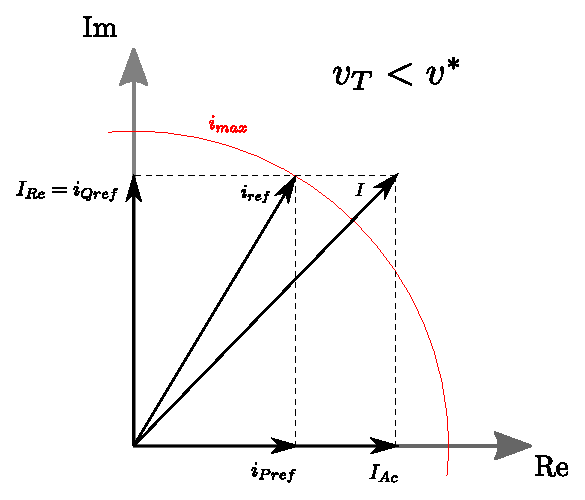
\includegraphics[width=\textwidth]{Images/priority_block2.eps}
		\caption{during voltage sag}
		\label{fig: priority_sag}
	\end{subfigure}
	\label{fig: CurrentPriority}
\end{figure}

Under normal conditions, the WPP must focus on delivering active power to the grid, as shown in Figure \ref{fig: priority_normal}. On the other hand, in the event of voltage sag, the WPP must act on the voltage regulation, providing as much reactive power as possible, as displayed in Figure \ref{fig: priority_sag}. Also, under no circumstances the current limitations of the components should not be violated.

The current priority block outputs the reference values of active and reactive current that will be used to control the power generated by the WPP. The following algorithm describes the current priority block operation.

\medskip

\begin{algorithmic}
	\IF {$\sqrt{I_{Ac}^{2} + I_{Re}^{2}} \leq i_{max}$}
		\STATE $i_{Pref} = I_{Ac}$
		\STATE $i_{Qref} = I_{Re}$
	\ELSE
		\IF {$v_{T} \geq v^{*}$}
			\STATE $i_{Pref} = min(i_{max}, I_{Ac})$
			\STATE $i_{Qref} = \sqrt{i_{max}^{2} - i_{Pref}^{2}}$
		\ELSE
			\STATE $i_{Qref} = min(i_{max}, I_{Re})$
			\STATE $i_{Pref} = \sqrt{i_{max}^{2} - i_{Qref}^{2}}$
		\ENDIF
	\ENDIF
\end{algorithmic}

At the next stage, proportional-integral blocks are used to represent the controllers of WTGs, specially the RSC controller. Their outputs follow the equations presented below. The values $V_{PA}$ and $V_{QA}$ are, respectively, the active and reactive voltage components (on grid coordinates) that the Thevenin voltage source must supply so the reference values of voltage and power are satisfied.

\begin{equation}
	\begin{cases}
		V_{PA} = k_{I}[(i_{Pref} - \frac{P}{v_{T}}) + \frac{1}{T_{I}}\int\displaylimits_{0}^{t} (i_{Pref} - \frac{P}{v_{T}})dt]\\
		\\
		V_{QA} = k_{I}[(\frac{Q}{v_{T}} - i_{Qref}) + \frac{1}{T_{I}}\int\displaylimits_{0}^{t} (\frac{Q}{v_{T}} - i_{Qref})dt]
	\end{cases}
	\label{eq: PI}
\end{equation}

At this point, the controllers operate on grid coordinates, so a coordinate transformation block is needed to adequate to $d-q$ coordinates. This block operates according to equation \eqref{eq: CoordShift}. It is important to notice that these equations rely on the knowledge of $\phi_{v}$ and, in order to obtain that measurement, the WPP must have a phasor measurement unit (PMU) installed on its substation.

\begin{equation}
	\begin{cases}
		V_{PAS} = -V_{PA}cos(\phi_{v}) - V_{QA}sin(\phi_{v}) \\
		V_{QAS} = V_{PA}sin(\phi_{v}) - V_{QA}cos(\phi_{v})
	\end{cases}
	\label{eq: CoordShift}
\end{equation}

Finally, limited lag blocks, simulating the delays caused by the electrical machine and converters present on WTGs, supply the voltage source. The lag block constraints limit the values of those voltage components to remain in a safety margin, between $0$ and $1$. Equation \eqref{eq: DelayBlocks} describes how these blocks affect $v_{D}$ and $v_{q}$.

\begin{equation}
	\begin{cases}
		\dot{v}_{d} = \frac{1}{T_{V}}(v_{d} - V_{PAS}) \\
		\dot{v}_{q} = \frac{1}{T_{V}}(v_{q} - V_{QAS})
	\end{cases}
	\label{eq: DelayBlocks}
\end{equation}

With direct and quadrature voltage components obtained, the power generated by the WPP can be easily calculated, as shown below.

\begin{align*}
		S^{*} &= v_{T}^{*} \cdot I = v_{T}^{*} \cdot \frac{[(v_{d} + jv_{q}) - v_{T}]}{R + jX} \\
		\\
		&= (v_{Td} - jv_{Tq})\cdot\left[\frac{v_{d} + jv_{q} - (v_{Td} + jv_{Tq})}{R + jX}\right]\cdot \frac{R - jX}{R - jX} \\
		\\
		&= \frac{v_{Td}v_{d} + v_{Tq}v_{q} - v_{T}^{2} + j(v_{Td}v_{q} - v_{Tq}v_{d})}{R^{2} + X^{2}}\cdot (R - jX) \\
		\\
		&= \frac{R(v_{Td}v_{d} + v_{Tq}v_{q} - v_{T}^{2}) + X(v_{Td}v_{q} - v_{Tq}v_{d})}{R^{2} + X^{2}} - j\frac{X(v_{Td}v_{d} + v_{Tq}v_{q} - v_{T}^{2}) - R(v_{Td}v_{q} - v_{Tq}v_{d})}{R^{2} + X^{2}} \\
\end{align*}

Thus,

\begin{equation}
	\begin{cases}
		P = \frac{R(v_{Td}v_{d} + v_{Tq}v_{q} - v_{T}^{2}) + X(v_{Td}v_{q} - v_{Tq}v_{d})}{R^{2} + X^{2}} \\
		Q = \frac{X(v_{Td}v_{d} + v_{Tq}v_{q} - v_{T}^{2}) - R(v_{Td}v_{q} - v_{Tq}v_{d})}{R^{2} + X^{2}}
	\end{cases}
	\label{eq: Outputs}
\end{equation}

The summary of the original model is shown below.

\begin{equation}
	\begin{cases}
		\dot{v}_{d} = \frac{1}{T_{V}}(v_{d} - V_{PAS}) \\
		\dot{v}_{q} = \frac{1}{T_{V}}(v_{q} - V_{QAS}) \\
		\\
		P = \frac{R(v_{Td}v_{d} + v_{Tq}v_{q} - v_{T}^{2}) + X(v_{Td}v_{q} - v_{Tq}v_{d})}{R^{2} + X^{2}} \\
		Q = \frac{X(v_{Td}v_{d} + v_{Tq}v_{q} - v_{T}^{2}) - R(v_{Td}v_{q} - v_{Tq}v_{d})}{R^{2} + X^{2}} \\
		\\
		V_{PAS} = -V_{PA}cos(\phi_{v}) - V_{QA}sin(\phi_{v}) \\
		V_{QAS} = V_{PA}sin(\phi_{v}) - V_{QA}cos(\phi_{v}) \\
		\\
		V_{PA} = k_{I}[(i_{Pref} - \frac{P}{v_{T}}) + \frac{1}{T_{I}}\int\displaylimits_{0}^{t} (i_{Pref} - \frac{P}{v_{T}})dt]\\
		V_{QA} = k_{I}[(\frac{Q}{v_{T}} - i_{Qref}) + \frac{1}{T_{I}}\int\displaylimits_{0}^{t} (\frac{Q}{v_{T}} - i_{Qref})dt]
	\end{cases}
	\label{eq: summary_original}
\end{equation}

\medskip

\begin{algorithmic}
	\IF {$\sqrt{I_{Ac}^{2} + I_{Re}^{2}} \leq i_{max}$}
		\STATE $i_{Pref} = I_{Ac}$
		\STATE $i_{Qref} = I_{Re}$
	\ELSE
		\IF {$v_{T} \geq v^{*}$}
			\STATE $i_{Pref} = min(i_{max}, I_{Ac})$
			\STATE $i_{Qref} = \sqrt{i_{max}^{2} - i_{Pref}^{2}}$
		\ELSE
			\STATE $i_{Qref} = min(i_{max}, I_{Re})$
			\STATE $i_{Pref} = \sqrt{i_{max}^{2} - i_{Qref}^{2}}$
		\ENDIF
	\ENDIF
\end{algorithmic}

\begin{equation*}
	\begin{cases}
		I_{Ac} = \frac{P_{ref}}{v_{T}} \\
		I_{Re} = k_{VC}(v_{Tref} - v_{T}) + \frac{Q_{ref}}{v_{T}}
	\end{cases}
\end{equation*}

Thus, this model can be interpreted as presented in \eqref{eq: xdot}, where the state variable ($x$), input ($u$), output ($y$) and parameter ($p$) vectors are described by \eqref{eq: x}, \eqref{eq: u}, \eqref{eq: y} and \eqref{eq: p}, respectively.

\begin{equation}
	\begin{cases}
		\dot{x} = f(x, y, p, u) \\
		y = g(x, p, u)
	\end{cases}
	\label{eq: xdot}
\end{equation}

\begin{equation}
	x = [v_{d}, v_{q}]^T
	\label{eq: x}
\end{equation}

\begin{equation}
	u = [v_{T}, \phi_{v}, P, Q]^T
	\label{eq: u}
\end{equation}

\begin{equation}
	y = [P, Q]^T
	\label{eq: y}
\end{equation}

\begin{equation}
	p = [R, X, k_{I}, T_{I}, T_{V}, k_{VC}, i_{max}]^T
	\label{eq: p}
\end{equation}

The parameters presented in \eqref{eq: p} are the subject of the estimation process presented on the next chapter. Those values define the behaviour of wind power plants during disturbances.

\subsection{Proposed Wind Power Plant Model for Further Studies}
\label{ssec: proposed_model}

One of the disadvantages of the model presented above is the need of information about voltage angle $\phi_{v}$. In order to acquire the voltage angle measurements, the grid must have special equipment, such as PMUs, installed in two of its buses, as shown in Figure \ref{fig: PMU_grid}. One of the PMUs must be located at the WPP terminal bus while the other must be installed at the slack bus\footnote{The slack bus is the bus used as angle reference in load flow studies} of the electrical power system. By processing the angle information provided by both equipment, the angle $\phi_{v}$ used on the estimation process is obtained.

\begin{figure}[h]
	\caption{Measurement of $\phi_{v}(t)$ with two PMUs installed on the grid}
	\begin{center}
		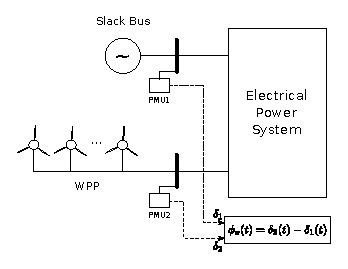
\includegraphics[scale=1.5]{Images/pmu_example.eps}
	\end{center}
	\label{fig: PMU_grid}
\end{figure}

However, the requirement of PMUs may limit the application of the original model \eqref{eq: summary_original} when these equipment are not available. One alternative to avoid that problem, proposed in this research, is to exclude the angle $\phi_{v}$ from the model equations. This can be obtained by dislocating the coordinate transformation block to the WPP terminal bus, as depicted in Figure \ref{fig: Proposed_Model}.

\begin{figure}[h]
	\caption{WPP model proposed in this research}
	\begin{center}
		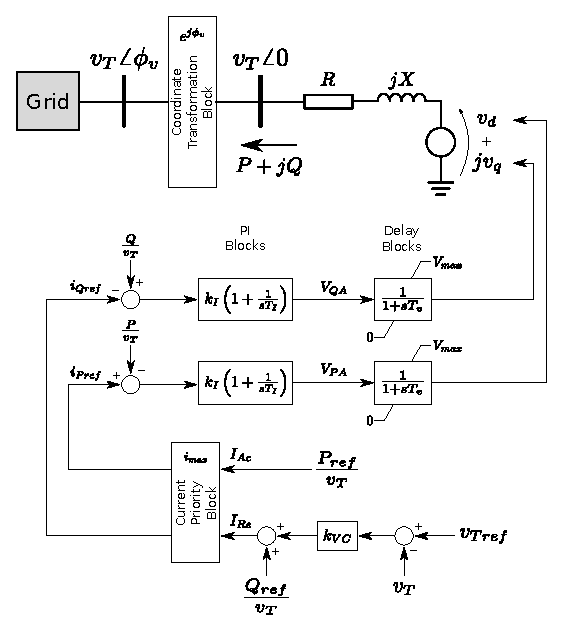
\includegraphics[scale=1]{Images/proposed_model.eps}
	\end{center}
	\label{fig: Proposed_Model}
\end{figure}

The model equations are slightly altered by this modification, as shown below by the summary of the proposed model. Moreover, the limits $V_{max}$ applied to the delay blocks also change, becoming parameters of the estimation process which demand further investigation.

\begin{equation}
	\begin{cases}
		\dot{v}_{d} = \frac{1}{T_{V}}(v_{d} - V_{PA}) \\
		\dot{v}_{q} = \frac{1}{T_{V}}(v_{q} - V_{QA}) \\
		\\
		P = \frac{R(v_{T}v_{d} - v_{T}^{2}) + Xv_{T}v_{q}}{R^{2} + X^{2}} \\
		Q = \frac{X(v_{T}v_{d} - v_{T}^{2}) - Rv_{T}v_{q}}{R^{2} + X^{2}} \\
		\\
		V_{PA} = k_{I}[(i_{Pref} - \frac{P}{v_{T}}) + \frac{1}{T_{I}}\int\displaylimits_{0}^{t} (i_{Pref} - \frac{P}{v_{T}})dt]\\
		V_{QA} = k_{I}[(\frac{Q}{v_{T}} - i_{Qref}) + \frac{1}{T_{I}}\int\displaylimits_{0}^{t} (\frac{Q}{v_{T}} - i_{Qref})dt]
	\end{cases}
	\label{eq: summary_proposed}
\end{equation}

\medskip

\begin{algorithmic}
	\IF {$\sqrt{I_{Ac}^{2} + I_{Re}^{2}} \leq i_{max}$}
		\STATE $i_{Pref} = I_{Ac}$
		\STATE $i_{Qref} = I_{Re}$
	\ELSE
		\IF {$v_{T} \geq v^{*}$}
			\STATE $i_{Pref} = min(i_{max}, I_{Ac})$
			\STATE $i_{Qref} = \sqrt{i_{max}^{2} - i_{Pref}^{2}}$
		\ELSE
			\STATE $i_{Qref} = min(i_{max}, I_{Re})$
			\STATE $i_{Pref} = \sqrt{i_{max}^{2} - i_{Qref}^{2}}$
		\ENDIF
	\ENDIF
\end{algorithmic}

\begin{equation*}
	\begin{cases}
		I_{Ac} = \frac{P_{ref}}{v_{T}} \\
		I_{Re} = k_{VC}(v_{Tref} - v_{T}) + \frac{Q_{ref}}{v_{T}}
	\end{cases}
\end{equation*}

The new state, input, output and parameter vectors are given by:

\begin{equation}
	x = [v_{d}, v_{q}]^T
	\label{eq: x_proposed}
\end{equation}

\begin{equation}
	u = [v_{T}, P, Q]^T
	\label{eq: u_proposed}
\end{equation}

\begin{equation}
	y = [P, Q]^T
	\label{eq: y_proposed}
\end{equation}

\begin{equation}
	p = [R, X, k_{I}, T_{I}, T_{V}, k_{VC}, i_{max}, V_{max}]^T
	\label{eq: p_proposed}
\end{equation}